\chapter{Обзор литературы}
\label{chap:lr}
\chaptermark{Обзор литературы}

\section{Традиционная архитектура компиляторов}
\label{sec:review_1}

С середины $20^{го}$ века исследования и индустрия разработки ПО сделали большой прорыв
в разработке компиляторов с акцентом на классическую задачу компиляции: 
создание быстрого и эффективного объектного кода для выполнения на виртуальной
машине или микропроцессоре.


Однако другие возможности компиляторов, такие как инструменты анализа кода, 
способные предоставлять исчерпывающую информацию о семантике программного кода,
остается необычным и редким качествои современных компиляторов для популярных языков программирования.

Наиболее наглядно эту проблему можно наблюдать в инструментах разработки для Java:

Код Java обычно компилируется с использованием компилятора Sun Java. "Будучи
монолитной программой, построенная по принципу ``черного ящика" \cite{Zouev2005}, 
Sun Java свособен лишь принять программный и сгенерировать из него байткод для виртуальной машины Java.


В то же время современная среда разработки включает в себя набор инструментов,
упрощающих работу программиста, и требует предварительного анализа синтаксиса и семантики кода, 
что не представляется возможным без построения Семантического Представления\cite{Zouev2005}. 
Построение такого представления требует реализовать основную функциональность компилятора заного.


Глядя в прошлое, легко понять причины этой проблемы: 
традиционно программы рассматривались как простые текстовые объекты
преобразующиеся в исполняемый код. Согласно этому предположению, компиляторы
были спроектированы очень логично: они не не хранили никакой информации о семантике исходного кода, 
помимов некоторых низкоуровневых внутренних промежуточных представлений.


Промежуточные представления этих компиляторов имели очень ограниченный набор вариантов использования \cite{Zouev2005, Zouev2010}, более того, они
хорошо подходили для единственной задачи: генерации объектного кода для числа поддерживаемых микропроцессоров. 
Также внутреннее представление компилятора нестабильно и имеет тенденцию очень активно меняться
во время разработки компилятора \cite{FreeSoftwareFoundation2016}. Следовательно, внутреннее представление компилятора не может 
быть использовано для построения средств анализа кода.

Ситуация с инструментарием C++ еще более удручающая: синтаксис языка
и семантика намного сложнее, чем у Java, поэтому создание альтернативного
компилятора --- весьма непростая задача даже для большого бизнеса.

В результате мы можем наблюдаеть заметный недостаток инструментов для C++\cite{Zouev2010}, а существующие
довольно сложны в реализации: среда разработки JetBrains CLion имеет собственный парсер
и семантический анализатор для реализации функций автодополнения, рефакторинга и статического анализа,
основанные на собственном семантическом представлении языка C++. 
Будучи сложным программным продуктом, парсер CLion, как правило, имеет собственные недостатки и 
отстает от развития языка на несколько месяцев после выхода нового стандарта.


Microsoft Visual Studio "страдает" от той же проблемы: VC++ генерирует промежуточное представление, пригодное
только для генерации кода: внутреннее представление сильно фрагментировано и очень низкоуровнево.
Набор инструментов C\&C++ IntelliSense в интегрированной среде разработки Microsoft Visual Studio 
полностью отделен от компилятора VC++ и реализует свой собственный парсер и семантический анализатор.

\section{Современные компиляторы и СП}
\label{sec:review_2}

Несмотря на то, что традиционные компиляторы сегодня широко используются, их
возможности по интеграции в среды разработки давно исчерпаны и всё больше новых языков сейчас
нацелены на реализацию семантического представления как стабильного промежуточного представления,
которое можно использовать во внешних инструментах семантического анализа.

Согласно \cite{Zouev2005, Zouev2010}, в отличие от промежуточного представления традиционного компилятора, 
семантическое представление содержит полный спектр ``знаний'' о программе, и включает в себя все аспекты, которые подразумеваются 
в исходном коде. Это дает возможность строить мощные инструменты, основанные на семантическом анализе.

\begin{itemize}
\item генерация кода
\item распределенная (или рекурсивная) проверка синтаксиса
\item человекопонятная визуализация
\item статический анализ
\item интерпретация программы
\item Семантический поиск: очень мощный метод запроса семантических объектов кода (пример: "найти все классы, производные от класса C, которые не переопределяют виртуальную функцию f”)
\end{itemize}

Существует три основных пути описания семантического представления и предоставления доступа к нему извне:
предоставление доступа к программному интерфейсу, который реализует доступ и модицикацию элементов семантического представления\cite{Cannon, FreeSoftwareFoundation2016}
отображение семантического представления на реляционную базу данных\cite{Linton1983},
и предоставление доступа к семантическому представлению в виде текста, используя открытый формат структурирования данных\cite{TheRustTeam2016}.

Цитируя \cite{Zouev2005}, ``API является универсальным способом реализации любой требуемой функциональности, 
но в условиях меняющихся требований, невозможно предугадать спектр потребностей клиентов''.
Открытый формат семантического представления, в свою очередь может стать решением потенциальной проблемы: ``Обычно доступ к открытому формату можно получить несколькими способами:
от простых API до высокоуровневых специалилированных программных продуктов. Кроме того, возможна реализация собственных инстерфейсов обработки семантического представления, выраженного в открытом формате''
And an open SP format can be a solution to potential problems: ``open formats

Конкретным форматом может являться как нечто собственной разработки, так и унифицированное стандартное решение, 
такое как XML\cite{Germon} или JSON\cite{ECMA-4042013}.

\newpage
\section{LSP and distributed approach to building development environment}
\label{sec:review_3}
Учитывая вышеизложенное, в настоящее время мы имеем прочную основу для обеспечения хорошего инструментария, 
основанного на семантическом анализе: методов представления семантического представления исходного кода программного обеспечения 
и его оценки в соответствии с потребностями клиентов.

Современные IDE применяют эти методы для предоставления достойного сервиса, но все же существует проблема: 
эти программные продукты используют свои собственные реализации компиляторов, обычно несвободные и не связанные с командой разработчиков исходного языка. 
Это подразумевает набор проблем, отмеченных в \ref{sec: review_1}.

Наличие хорошего современного компилятора, способного генерировать SR, делает вещи немного менее сложными, 
но все же не решает проблему времени и стоимости реализации IDE для конкретного языка.

Очевидно, что эти проблемы не являются уникальными для класса продуктов IDE, но для любой большой монолитной архитектуры, 
и решение может быть довольно простым: если мы можем снизить связывание системы и представить среду разработки в виде набора инструментов 
вместо одного интегрированного решения, мы можем распределить реализацию IDE, чтобы иметь набор несвязанных модулей:
\begin{itemize}
    \item An editor
    \item Compiler to SR
    \item SR clients (described in \ref{sec:review_1})
    \item Protocol between an editor and the language-specific part
\end{itemize}
\newpage

\begin{figure}[H]
    \centering
    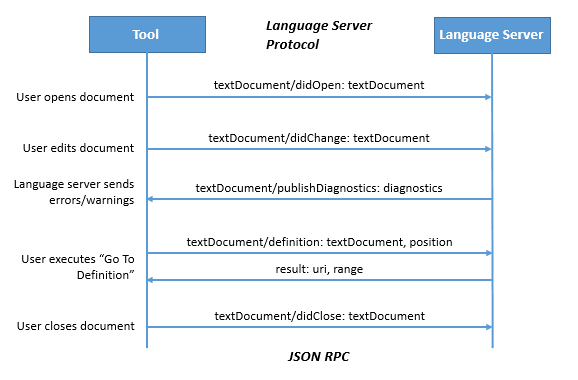
\includegraphics[width=0.85\textwidth]{figs/lsp.png}
    \caption{Language Server Protocol}
\end{figure}

The last one have not been introduced yet: the protocol to connect any
third-party tool to the language infrastructure, achieving a decent IDE-like
functionality without its maintenance and development costs

Language Server and Language Server Protocol introduced by Microsoft in 2016
represent a development environment as two disjoint parties:
\begin{itemize}
    \item Language Servers to implement all the SR analysis things
    \item Clients as editors or other development tools using the LSP to communicate with Language Servers \cite{Sourcegraph}
\end{itemize}

\section{Conclusion}
\label{sec:review_conclusion}

Conventional compilers with a monolithic architecture, that are only good at executable code generation,
are hard to integrate into a modern development environment as they do not share
semantic representation of the source code, thus to develop a good IDE one must write their own
source code to Semantic Representation compiler.

A modern compiler (that does share a high-level intermediate representation) is
a big step towards simpler language toolings and it can become even more convenient
combined with a distributed IDE architecture that splits an editor and the language toolchain
into two disjoint parts, linking them via a standardized protocol.

This approach gives language developers a great opportunity to make use of an
existing development infrastructure, providing their Language Server for a
giant set of development tools, as well as a way to fearlessly experiment with new and
existing analysis techniques, e.g. a Software Knowledge Base\cite{Wanghong}, described by
Bertrand Meyer, may be implemented as a language server module, as an
alternative approach to the one selected by the original author in 1985:
integration of analysis tool into an editor was not possible back then, but this is
the exact thing that LSP is good for now.

Concluding, the Language Server may be considered to be the most feasible
solution to rapidly bootstrap rich development infrastructure for aspiring new
languages, with a broad path to evolve further.